\clearpage
\chapter{Advanced Harmony: Sevenths, Voice Leading and Reharmonisation}
\label{chap:advanced-harmony}

\subsection*{What you can do after this chapter}
\begin{itemize}
  \item Distinguish dominant, major, minor, half-diminished and diminished sevenths by construction and function, instead of treating ``seventh chord'' as one colour.
  \item Check four-part writing with common tones, stepwise motion and resolution, and point out parallel fifths/octaves or an unresolved seventh.
  \item Use inversions, drop-2, a pedal bass and sequential reharmonisation to make three versions of one melody.
  \item In Yeban, turn an eight-bar I--vi--IV--V into ii--V--I and a borrowed-chord version, then compare bass line and tension.
\end{itemize}

\subsection{The five qualities of seventh chords}

A seventh chord = triad + seventh. Its quality is fixed by the intervals from the root to the third, fifth and seventh:

\begin{center}
\small
\begin{tabular}{clll}
\toprule
Quality & Construction (semitones) & Symbol & Typical position \\
\midrule
Dominant seventh & 4, 7, 10 & X7 & V7; blues I7/IV7 \\
Major seventh & 4, 7, 11 & Xmaj7 & Imaj7, IVmaj7 \\
Minor seventh & 3, 7, 10 & Xm7 & ii7, vi7, iii7 \\
Half-diminished & 3, 6, 10 & Xm7\(\flat\)5 & viiø7, iiø7 (minor) \\
Diminished seventh & 3, 6, 9 & Xdim7 & passing/symmetric tension, rarely a stable tonic \\
\bottomrule
\end{tabular}
\end{center}

The most common functional cell is ii7--V7--Imaj7: ii7's minor seventh contains the tonic's sixth, V7's tritone (3 and \(\flat\)7) points at I, and Imaj7's major seventh pins the arrival. Do not treat V7's \(\flat\)7 as decoration: it must descend stepwise to the third of I, or the arrival feels suspended.

\subsection{Voice leading: three hard rules and two soft rules}

Four-part writing (SATB or four instruments) reads horizontally first, vertically second. Hard rules:

\begin{enumerate}
  \item \textbf{Resolve the seventh}: V7's seventh descends stepwise to the third of I; ii7's seventh descends to the third of V7.
  \item \textbf{Resolve the leading tone}: V7's third (the major leading tone) rises to the tonic of I; in an inner voice it may fall to the fifth, but never leap.
  \item \textbf{No parallel fifths/octaves}: two voices moving in similar motion from one perfect fifth/octave to another weaken independent part-writing.
\end{enumerate}

Soft rules:

\begin{itemize}
  \item Prefer common tones, then stepwise motion, then leaps; after a leap, compensate with a step in the opposite direction.
  \item Let bass and melody move in contrary motion; avoid simultaneous large leaps in outer voices.
  \item Double roots and fifths first; avoid doubling the third (leading tone) and the seventh.
\end{itemize}

\begin{figure}[htbp]
\centering
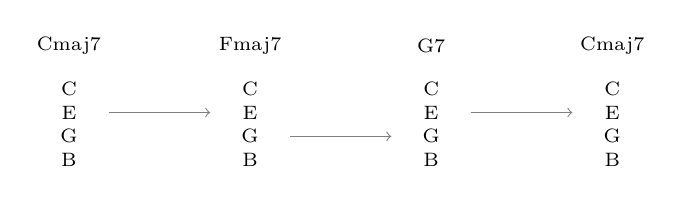
\begin{tikzpicture}[x=2.3cm,y=0.55cm,font=\scriptsize]
  \foreach \x/\ch/\n in {0/Cmaj7/{C E G B},1/Fmaj7/{F A C E},2/G7/{G B D F},3/Cmaj7/{C E G B}} {
    \node at (\x,2.6) {\ch};
    \foreach \i/\t in {0/C,1/E,2/G,3/B} { \node at (\x,1.6-\i*0.55) {\t}; }
  }
  \draw[->,gray] (0.22,1.05)--(0.78,1.05);
  \draw[->,gray] (1.22,0.5)--(1.78,0.5);
  \draw[->,gray] (2.22,1.05)--(2.78,1.05);
\end{tikzpicture}
\caption*{Figure 11-1: Common tones and steps in Cmaj7--Fmaj7--G7--Cmaj7. Keep common tones when possible and move the rest by the smallest step; G7's F falls to Cmaj7's E, B rises to C.}
\end{figure}

\subsection{Inversions, drop-2 and the bass line}

An inversion changes the bass (third, fifth or seventh), not the chord quality. Fix the bass line first, then choose the inversion:

\begin{itemize}
  \item \textbf{First inversion}: third in the bass; useful for stepwise bass (C--E--G--B).
  \item \textbf{Second inversion}: fifth in the bass; common as a passing chord or over a pedal.
  \item \textbf{Drop-2}: lower the second-highest voice by an octave for a more open keyboard/guitar voicing; check that it does not collide with the bass.
\end{itemize}

Example: C--F--G--C with bass C--F--G--C makes fourth leaps; C--F/A--G/B--C gives a stepwise C--A--B--C, but do not park F/A's second inversion for long.

\subsection{Reharmonisation: three ways with the same melody}

Reharmonisation is not ``replace everything with strange chords''; it changes how the harmony interprets the melody. Three controllable devices:

\begin{enumerate}
  \item \textbf{Functional substitution}: I may become vi or iii; IV may become ii; V may become viiø7 or a substitute dominant. The bass and melody must still read as the same function.
  \item \textbf{Pedal bass}: keep the bass fixed and change the upper chords, producing ``same root, different colours''; useful in intros and bridges.
  \item \textbf{Sequential reharmonisation}: move the same motivic harmony down/up a second or third while preserving voice relationships; after two sequences, return, or it becomes an exercise.
\end{enumerate}

\begin{center}
\small
\begin{tabular}{clll}
\toprule
Original & Substitution & Sound & Risk \\
\midrule
I--vi--IV--V & ii--V--I--vi & jazzier, descending bass & ii7's seventh must resolve \\
I--IV--V--I & I--IV--ii--V & smoother, delays the tonic & count the ii--V seventh chain \\
I--V--vi--IV & I--V--vi--IV (borrow Fm) & darker, pre-chorus contrast & Fm must return to C \\
\bottomrule
\end{tabular}
\end{center}

In Yeban: split eight bars in half, I--vi--IV--V then ii--V--I--V; solo each bar's bass. If the bass leaps more than a fourth, fix it with inversions before adding colour.

\subsection{Exercises}

\begin{exercise}
\begin{enumerate}
  \item Write the four notes of C major V7 and say where the seventh and third resolve.\\
  \emph{Answer:} G B D F; F falls to E, B rises to C.
  \item Why may V7's third fall in an inner voice while the leading tone in an outer voice usually rises?\\
  \emph{Answer:} The outer-voice leading tone has the strongest pull; an inner voice may fall to the fifth to avoid voice crossing, but still may not leap.
  \item Write a stepwise bass for C--F--G--C and mark the inversions.\\
  \emph{Sample:} C--F/A--G/B--C; F in first inversion, G in first inversion.
  \item Change I--vi--IV--V to ii--V--I--vi and name every seventh that must resolve.\\
  \emph{Answer:} ii7's seventh falls to V7's third; V7's seventh then falls to I's third.
  \item Harmonise a four-bar C major melody over a pedal C; write the upper chords.\\
  \emph{Sample:} pedal C, upper Cmaj7--Fmaj7/C--Dm7/C--G7/C.
  \item In Yeban, lay eight bars of I--vi--IV--V with bass C--A--F--G, then change the first half to ii--V--I--vi; compare the bass leaps and seventh resolutions.\\
  \emph{Sample:} the original bass C--A--F--G has third/fourth leaps; the rewrite C--D--C--A is more stepwise, but ii7's seventh must fall to V7's third, not stop on the bar line.
\end{enumerate}
\end{exercise}

\subsection{Help topic mapping}
\begin{center}
\footnotesize
\setlength{\tabcolsep}{3pt}
\begin{longtable}{p{0.34\linewidth}p{0.45\linewidth}p{0.15\linewidth}}
\toprule
Section & In-app help anchor & Note \\
\midrule
\endhead
Seventh-chord qualities & \texttt{music-theory-seventh-chords} & Table 11-1 \\
Voice-leading rules & \texttt{music-theory-voice-leading} & Figure 11-1 \\
Inversions and bass line & \texttt{music-theory-inversions-bass} & Operation \\
Three reharmonisation devices & \texttt{music-theory-reharmonisation} & Table 11-2 \\
How to do it in Yeban & \texttt{music-theory-reharmonise-eight-bars} & Operation \\
Exercises & \texttt{music-theory-ch11-practice} & Answers in this chapter \\
\bottomrule
\end{longtable}
\end{center}
